\documentclass[]{IEEEtran}
\usepackage[utf8]{inputenc}
\usepackage[english]{babel}

\title{Scooter Trajectories Clustering\\
	{\large University of Verona\\Computer Engineering for Robotics and Smart Industry\\Machine Learning and Deep Learning\\2020/2021\\}}
\author{Mirco De Marchi - VR445319}

%\usepackage{algorithm,algorithmic}

\usepackage{hyperref}
\hypersetup{
    linktoc=all
}

\usepackage{graphicx}
\graphicspath{ {images/} }

\usepackage{listings}

% Table environment
\usepackage{tabularx}
\renewcommand{\arraystretch}{1.2}
\usepackage{float}
\restylefloat{table}

\usepackage{amsmath}

\usepackage{tikz}
\usetikzlibrary{positioning,shapes,shadows,arrows}

\usepackage{multicol}
%\setlength{\multicolsep}{6.0pt plus 2.0pt minus 1.5pt}% 50% of original values
\setlength\multicolsep{0pt}

\begin{document}
\maketitle

% ABSTRACT
\begin{abstract}
	The aim of this review is to present the main unsupervised learning techniques used for scooter trajectories clustering. The dataset that I used contains a big amount of positions taken in rentals that run through some cities in Italy. The objective is to find recurrent places crossed by the trajectories. This review presents some analysis on the positions and the implementation of some heuristics that manage data in a systematic way: the \textit{spreaddelta heuristic}, the \textit{edgedelta heuristic} and the \textit{coorddelta heuristic}. Then I performed some machine learning clustering techniques on the dataset: \textit{mean shift}, \textit{full linkage}, \textit{ward hierarchical} and \textit{k-means}, adding the features extracted from the heuristics performed before. All the features are extracted with \textit{Principal Component Analysis (PCA)} with an improvement that select the component to focus on and the features has been integrated with the informations obtained from the heuristic procedures in order to optimize feature extraction. 
\end{abstract}

% INTRODUZIONE
\section{Motivation}
Motion trajectories are really difficult to analyse and handle because of the amount of data. There could be errors in position tracking and usually you don't have informations like the city from which the positions are taken, or any higher semantic level information that can help in trajectories grouping. Consequently trajectories are difficult to represent, filter and manage in relation with itself or other data. First of all, trajectories clustering is a challenge for its intrinsic difficulty in being treated and today is an ambitious topic in data science research. Moreover trajectory clustering can help for several applications:
\begin{itemize}
	\item Monitoring: understand main points of interest and common places visited by tourists;
	\item Forecasting: prediction of possible destinations starting from a position; 
	\item Viability: traffic monitoring and detection of possible point of traffic jam;
\end{itemize}


% BACKGROUND
\section{State of art}
\textit{Yuan et al. (2012)} \cite{AIReview}, in their trajectory clustering review, show some techniques widely used for moving object clustering. The latest Machine Learning algorithms are all evolution and improvement of the traditional clustering techniques: K-Means, Mean Shift, Gaussian Mixture, Hierarchy, Agglomerative, etc. For spacial based clustering, \textit{Palma et al. (2008)} \cite{Palma2008} considers trajectories geometrical properties to detect pauses and moves in trajectories by using an improved version of \textit{DBSCAN} algorithm. For time depended clustering, \textit{Nanni and Pedreschi (2006)} \cite{Nanni2006} considers time gaps between trajectory positions and proposes \textit{T-OPTICS} as an adaption of \textit{OPTICS}. For partition based clustering, \textit{Lee et al. (2007)} \cite{Lee2007} implement a \textit{partition \& group} framework for trajectory clustering based on a formal theory. For uncertain trajectory clustering, Nock and Nielsen 2006 \cite{Nock2006} implemented \textit{Fuzzy C-Means (FCM)} that model the uncertainty and reduce the noise of trajectories location between discrete time updates. For semantic trajectory clustering, several works start considering geographical informations as a background from which extracting higher semantic level information (\textit{Palma et al. (2008)} \cite{Palma2008} stops and moves).

On the other hand, the main Deep Clustering techniques are based on autoencoders and was first introduced with the \textit{D. Yao et al. (2017)} \cite{DeepLearningRepresentation} work, in which they present a technique based on a sliding window that extract behavior feature along the trajectories and further employ a sequence to sequence autoencoder to learn fixed-length deep representation. The autoencoder based clustering, introduced in \textit{D. Yao et al. (2017)} \cite{DeepLearningRepresentation} work, reduces the trajectory representation in a latent space contained in the neural network architecture, but then a traditional clustering algorithm has to be applied in order to locate similar trajectories. \textit{Olive et al. (2020)} \cite{DeepLearningAutoencoders} employs a deep clustering method named \textit{DCEC (Deep Convolutional Embedded Clustering)}, that uses a convolutional autoencoder and it can identify the clusters directly without the need of using a classical clustering method. In the same work (\cite{DeepLearningAutoencoders}) they implement \textit{artefact}, a method based on a feed-forward autoencoder and a loss function combining the reconstruction error and a regularisation term based on the projection operator \textit{t-SNE}. \textit{M. Yue et al. (2019)} \cite{DETECT} have currently produced the best deep clustering solution that is named \textit{DETECT (Deep Embedded TrajEctory ClusTering network)}. \textit{DETECT} operates in three parts: first it transforms the trajectories by selecting its own point-of-interest for each position based on its context derived from their geographical locality, then they use autoencoder to learn trajectory representation and finally the a clustering oriented loss is directly built on the latent space features to refine the cluster assignment.

Furthermore, there are works on Deep Clustering that do not adopt the autoencoder architecture. \textit{Mahdi M. K. et al. (2015)} \cite{MotionPatternApproach} proposed an algorithm composed by four phases in which they break down trajectories into flow vectors that indicate instantaneous movements and then they apply different clustering steps in order to extract similarity with respect to their location, velocity, spacial proximity, motion and reachability. \textit{Manduchi L. (2020)} \cite{DPSOM} present \textit{DPSOM (Deep Probabilistic Clustering with Self-Organizing Maps)}, that is based on the \textit{SOM (self-organizing-map)}, which is a clustering technique that creates a nuance between the boundaries of the cluster, thus giving a more flexible interpretation of the clusters. In particular the \textit{T-DPSOM} algorithm outperforms baseline methods in time series clustering and time series forecasting.

In this report I will present some partition and group heuristics, based on time gaps, I will show how the traditional clustering algorithms can be used for trajectory clustering relying on positions spatial information and I will compare the results with Deep Clustering techniques based on the autoencoder architecture explained in \cite{DeepLearningRepresentation}. 


% METODOLOGIA
\section{Objectives}
The objectives of this project is grouping trajectories in order to find common locations crossed by people that rent a scooter to visit a city in Italy. The model built has to be able to distinguish for example the positions related to a trajectory that takes from the train station to the city centre, the ones that move in the city centre, the ones that run through the periphery and so on.

% METHODOLOGY
\section{Methodology}
\subsection{Dataset}

The original dataset is composed by 4 tables in CSV fomat: \textit{pos.csv}, \textit{rental.csv}, \textit{user.csv}, \textit{device.csv}. This dataset is a subset of another dataset with some sensitive data dropped (like user name or email) and positions manumit in order to protect proprietary data. Although this dataset is only a subset of the proprietary data, the positions amount is really huge and it weighs about 2GB. 

The \textit{pos.csv} table contains all the positions, characterized by latitude, longitude, speed, timestamp and a rental id used to join with \textit{rental.csv} table. The \textit{device.csv} and \textit{user.csv} tables contain the kilometres travelled respectively by a scooter and by a user. At last, the \textit{rental.csv} table contains the start position and end position in couple of longitude and latitude of the rental trajectories with related start and stop timestamps, and the ids used to join the device and user tables. The dataset was subsequently reorganized, filtered and sorted in such a way to have positions in relation with its rental and the positions that belongs in the range of rental start-end time. This operation was really tricky because the total amount of data is huge and I had to optimize database join algorithms and chunks management to be able to handle these data in acceptable time, but in the end the resulting dataset properties diagram is \ref{generated-dataset-diagram}. The figure \ref{fig:starting-point} shows all positions in the two Italy cities contained in \textit{pos.csv} table.

\begin{figure*}[bt]
	\centering
	\includegraphics[width=\textwidth]{starting-point}
	\caption{Trajectories without clustering in 2 Italy cities}
	\label{fig:starting-point}
\end{figure*}

Due to how the dataset is constructed, a trajectory can initially be represented as a set of positions $trajectory = \{p_1, p_2, p_3, ..., p_t\}$ that belong to the same rental sorted by the timestamp. Each position $p$ is a tuple $(t_p, lat_p lon_p, s_p)$ where $t_p$ is the server timestamp or the device timestamp, $lat_p$ and $lon_p$ are the longitude and the latitude of the position and $s_p$ is the speed. Formally a trajectory is $trajectory(rental\_id) = \{ p \mid p.rental\_id == rental\_id  \}$ and $TRAJ$ is the set of all trajectories \ref{fig:trajectory-rental}. The resulting figure of the trajectory divided in rental is \ref{fig:rental-plot}.

\begin{figure}[bt]
	\centering
	\includegraphics[width=\columnwidth]{trajectory-rental}
	\caption{Trajectories belonging rentals}
	\label{fig:trajectory-rental}
\end{figure}

\begin{figure*}[bt]
	\centering
	\includegraphics[width=\textwidth]{rental-plot}
	\caption{Trajectories belonging rentals}
	\label{fig:rental-plot}
\end{figure*}

\subsection{Heuristics}

After that, I performed some analysis on features. I studied their distribution and I started to think how could be possible to group or divide positions. Two trajectories can be similar in shape and can be divided in time. It means that a sequence of positions, a trajectory, can be similar to another one, evaluating his shape appearance and location in the geographical map, and therefore his sequence of their geographical coordinates. On the other hand, a trajectory can be different to another one if there is a temporal space between each other. 

\begin{table}
	\centering
	\caption{Number of features and samples of generated dataset}
	\begin{tabular}{ l r r }
		\hline
		Dataset & Samples & Features \\ \hline
		rental & 14826 & 10 \\ 
		pos & 817076 & 18 \\ 
		merge & 817076 & 18 \\
		dataset & 14826 & 13 \\
		partition city 1 & 608251 & 18 \\
		partition city 2 & 202795 & 18 \\ \hline
	\end{tabular}
\end{table}

As result I implemented 3 different clustering heuristics performed in a systematic and statistical way on the entire sequence of positions:
\begin{itemize}
	\item \textbf{timedelta heuristic}: considers that a trajectory of a rental can be divided in a sequence of trajectories if the time gap between a position and previous one exceeds a \textit{timedelta} value. First of all I calculated the time gaps for each set of positions grouping in rental: 
	\begin{align}
		TIMEGAPS = \{t.time - shift(t, -1).time \mid \forall t \in TRAJ \}
	\end{align}
	where \verb|shift(t, -1)| shifts the trajectory backward and the field \verb|.time| gives the timestamp of each position in trajectory. The \textit{timedelta} value has been manually assigned or automatically calculated with the statistical empirical rule (three-sigma rule or 68-95-99.7 rule). The timegaps set is then used to divide the trajectories if the gap exceeds the defined timedelta (figure \ref{fig:trajectory-timedelta}).
	
	\begin{figure}[bt]
		\centering
		\includegraphics[width=\columnwidth]{trajectory-timedelta}
		\caption{Trajectories belonging timedelta heuristic}
		\label{fig:trajectory-timedelta}
	\end{figure}
	
	\item \textbf{spreaddelta heuristic}: considers that a rental trajectory can be considered similar to another one if they spread a similar amount of area (figure \ref{fig:spreaddelta-pred}). I calculate the spread area for each rental trajectory in the following way: 
	\begin{align}
		SPREADS = \{max(t) - min(t) \mid \forall t \in TRAJ \}
	\end{align}
	where \verb|max(t)| and \verb|min(t)| calculate respectively the maximum and the minimum latitude and longitude of a set of positions, and \verb|TRAJ| is the set of trajectories that can be grouped for each rental or for the \textit{timedelta heuristic} (figure \ref{}). Also in this case, I exploited the empirical rule to compute the spreaddelta value. 
	
	\begin{figure}[bt]
		\centering
		\includegraphics[width=\columnwidth]{spreaddelta-pred}
		\caption{For spreaddelta heuristic $Traj1$ and $Traj4$ are similar because they spread a similar amount of area}
		\label{fig:spreaddelta-pred}
	\end{figure}

	\begin{figure}[bt]
		\centering
		\includegraphics[width=\columnwidth]{spreaddelta-calc}
		\caption{Spreads calculus in trajectory}
		\label{fig:spreaddelta-calc}
	\end{figure}
	
	\item \textbf{edgedelta heuristic}: acts as the \textit{spreaddelta heuristic}, but it considers the edges of a trajectory, or rather the first position and the last position of a trajectory \ref{fig:edgedelta-pred}. The main problem here is that the distribution of edge positions has 2 centres or, in other words, it is bimodal. To resolve this issue I applied for simplicity only 1 iteration of \textit{Mean Shift} starting from a random position in order to get closer to one of 2 centre. The set of edges is calculated in the following way (figure \ref{fig:edgedelta-calc}): 
	\begin{align}
		EDGES = \{concat(p[0], p[-1]) \mid \forall t \in TRAJ \}
	\end{align}
	
	\begin{figure}[bt]
		\centering
		\includegraphics[width=\columnwidth]{edgedelta-pred}
		\caption{For edgedelta heuristic $Traj1$ and $Traj4$ are similar because they start and finish nearly}
		\label{fig:edgedelta-pred}
	\end{figure}
	
	\begin{figure}[bt]
		\centering
		\includegraphics[width=\columnwidth]{edgedelta-calc}
		\caption{Edges calculus in trajectory}
		\label{fig:edgedelta-calc}
	\end{figure}

	\item \textbf{coorddelta heuristic}: it is a combination of spread and edge heuristics in order to combine the main advantages of each other. 
\end{itemize}

\subsection{Feature extraction}

For feature extraction I decided to perform \textit{Standardization}, \textit{Normalization} and than \textit{Principal Component Analysis (PCA)}.

As feature extraction, I considered that the work done for the heuristic algorithms could return useful for clustering algorithms. In particular $TIMEGAPS$, $SPREADS$ and $EDGES$ sets can be used as new features for my data. Therefore, I integrate my data features with the heuristic values and I run the pipeline of \textit{Standardization}, \textit{Normalization}, \textit{PCA} and than clustering algorithms. In particular, I tried to perform this pipeline with space and time features together, with only space features, and then with space and heuristic features together. Moreover I tried to perform clustering algorithm on the whole trajectories and even on one city at a time.

The feature extraction algorithm for Deep Clustering is the behavior feature extraction. The key idea of the behavior feature extraction is to utilize a sliding window to traverse the records and extract features in each window. As shown in \ref{fig:moving-behavior-feature}, with a sliding window, we aim to obtain space- and time- invariant features to describe the moving behaviors of the object.

\begin{figure}[bt]
	\centering
	\includegraphics[width=\columnwidth]{moving-behavior-feature}
	\caption{Moving behavior feature extraction algorithm}
	\label{fig:moving-behavior-feature}
\end{figure}

Let $L$ and $offset$ denote the width and the offset of the sliding window, respectively. While classic methods often choose $offset = L$, a finer granularity of $offset= 1/2 * L$ can effectively lead to better performance. 
The moving behavior changes can be reflected by the differences of the attributes between two consecutive records. Let us consider a window with $L$ records. The records in this window are denoted as $W = (p_1, p_2, ..., p_i, ..., p_L)$. 
Assume the attributes in each record consist of speed and rate of turn (ROT). The extracted attributes for the moving behaviors include: time interval $\Delta t_i = t_{p_i} - t_{p_{i-1}}$, change of position $\Delta lat_i = lat_{p_i} - lat_{p_{i-1}}$ and $\Delta lon_i = lon_{p_i} - lon_{p_{i-1}}$, change of speed $\Delta s_i = s_{p_i} - s_{p_{i-1}}$ and change of ROT $\Delta r_i = r_{p_i} - r_{p_{i-1}}$, where $i$ ranges from 2 to $L$. 

In this way, a window with $L$ records has $L-1$ moving behavior attributes of kind $(\Delta lat, \Delta lon, \Delta s, \Delta r)$.
If $L => 1$, for each $i$ from 1 to $L-1$, we compute $\Delta t_i$, $\Delta lat_i$, $\Delta lon_i$, $\Delta s_i$ and $\Delta r_i$. Further compute the change rate of these features $f_i = (f_{\Delta lat_i}, f_{\Delta lon_i}, f_{\Delta s_i}, f_{\Delta r_i})$ in which $f_{\Delta lat_i} = \Delta lat_i / \Delta t_i$, $f_{\Delta lon_i} = \Delta lon_i / \Delta t_i$, $f_{\Delta s_i} = \Delta s_i$, $f_{\Delta r_i} = \Delta r_i$. For two consecutive records, $f_{\Delta lat_i}$ and $f_{\Delta lon_i}$ stand for the average speed, $f_{\Delta s_i}$ stands for the change of speeds and $f_{\Delta r_i}$ stands for the change of ROTs. After computing these features in each pair, we get a feature set $f = {f1, f2, ..., f_{L-1}}$. We use the statistic of f to generate the features in the sliding window. Here, six statistics ${mean, max, 75\%quantile, 50\%quantile, 25\%quantile, min}$.

In summary, the moving behavior features of each window has $4 * 6 = 24$ dimensions that consist of ${f_{\Delta lat}, f_{\Delta lon}, f_{\Delta s}, f_{\Delta r}} \times {mean, max, 75\%quantile, 50\%quantile, 25\%quantile, min}$.
If $R = 0$,  skip this window. Algorithm 1 shows the generation procedure of moving behavior feature sequence.
For each trajectory in $T$, we generate the moving behavior sequence for it. Then, we put these sequences in a set and denote it as $BS = {BTR1,BTR2,...,BTRN}$. Finally, we normalize each feature to prepare for the next sequence to sequence auto-encoder layer.

\subsection{Clustering}

The clustering algorithms that I used are the following: 
\begin{itemize}
	\item \textit{K-Means}: choose centroids that minimise the \textit{inertia}, or \textit{within cluster sum of squares (WCSS)} criterion.
	\item \textit{Mean Shift}: discover blobs in a smooth density of samples with the purpose to find the mean of points within a given region. 
	\item \textit{Gaussian Mixture}: implements the \textit{expectation-maximization (EM)} algorithm for fitting mixture of Gaussian models. 
	\item \textit{Full and Ward Hierarchy Agglomerative}: hierarchical clustering using a bottom up approach and minimizes the maximum distance between observations in pairs of clusters (Full) or minimizes the sum of squared differences between all clusters (Ward). 
\end{itemize}

\subsection{Deep Clustering}

An autoencoder is a type of deep neural network used to learn efficient codings of unlabeled data (unsupervised learning). The encoding is validated and refined by attempting to regenerate the input from the encoding. The autoencoder learns a representation (encoding) for a set of data, typically for dimensionality reduction, by training the network to ignore insignificant data (Figure \ref{fig:autoencoder-schema}). 

\begin{figure}[bt]
	\centering
	\includegraphics[width=\columnwidth]{autoencoder-schema}
	\caption{Autoencoder main principle}
	\label{fig:autoencoder-schema}
\end{figure}

The LSTM autoencoder models used are the following:
\begin{itemize}
	\item \textit{Simple Autoencoder}: the model is composed by an LSTM that which acts as encoder and another LSTM that acts as decoder. Initially the state of the encoder LSTM is randomly initialized. During training process, the output generated from the encoder is passed to the decoder and the LSTM decoder state is initialized with the encoder one (figure \ref{fig:lstm-autoencoder-schema}). 
	
	\begin{figure}[bt]
		\centering
		\includegraphics[width=\columnwidth]{lstm-autoencoder-schema}
		\caption{Simple Autoencoder schema}
		\label{fig:lstm-autoencoder-schema}
	\end{figure}

	\item \textit{Autoregressive Autoencoder}: the encoder LSTM reads the input sequence sequentially and the hidden state $state_i$ is updated accordingly. After the last position of the trajectory is processed, the hidden state $state_t$ is used as the representation for the whole sequence. Then, the decoder first generates the output by taking $state_t$ as the initialized hidden state of the decoder LSTM and the last output of the encoder as the first input of the decoder, and then further generate the other output taking as input the previous output, so as to form the following autoregressive model \ref{fig:autoregressive-autoencoder-schema}.
	\item \textit{Addons Autoencoder}: the model is the same of the previous one, but the decoder part is substitute with an already implemented decoder contained in \textit{TensorFlow Addons} library. The decoder is named \texttt{BasicDecoder} and it is trained with the \texttt{TrainingSampler} that reads output distribution of the current decoding step and pass it to the next decoding step (figure \ref{fig:autoregressive-autoencoder-schema}).
	
	\begin{figure}[bt]
		\centering
		\includegraphics[width=\columnwidth]{autoregressive-autoencoder-schema}
		\caption{Autoregressive Autoencoder schema}
		\label{fig:autoregressive-autoencoder-schema}
	\end{figure}
\end{itemize}

The target of the decoder is to reconstruct the input sequence. In other words, the encoder LSTM and decoder LSTM are trained together by minimizing the reconstruction error. 

The input target of the LSTM autoencoder models could be the moving behavior features but also the raw positions features. In fact, a fundamental characteristic of the neural networks is to learn well the trend of the training inputs, consequently in this case it is not essential to apply a feature transformation algorithm when there are already many. 

In order to reproduce the sliding window behavior when raw positions are used, the training is performed creating a dataset of sliding windows over the input timeseries trajectory. Then, the input shape for the autoencoder becomes $batch_size \times number_of_sliding_window \times sliding_window_width $.

% RESULTS
\section{Results}
The best way to show the clustering results is plotting the trajectory with different colours in relation to the cluster which it belongs. In addiction, for clustering algorithms, I used a method of interpretation and validation of consistency within clusters of data, called \textit{Silhouette}. 

\textit{Silhouette} clustering validation technique measures how similar an object is to its own cluster compared to other clusters. The silhouette ranges from -1 to +1, where a high value indicates that the object is well matched to its own cluster and poorly matched to neighbouring clusters.

The results of heuristic analysis are the following: 
\begin{itemize}
	\item \textit{timedelta heuristic}: in figure \ref{fig:timedelta-result} you can see some rentals with their positions divided in subgroups of trajectories. That sub trajectories are built considering only the time gaps between the positions, no latitude or longitude has been used to produce this result. This result shows how the time sequences could be really useful to produce a good trajectory partition.
	
	\begin{figure}[bt]
		\centering
		\includegraphics[width=\columnwidth]{timedelta-result}
		\caption{Timedelta heuristic line plot in details}
		\label{fig:timedelta-result}
	\end{figure}
	
	\item \textit{spreddelta heuristic}: in figure \ref{fig:spreaddelta-result} you can see how the trajectories are clusterized in 3 main groups: wide area trajectories (green), medium area trajectories (blue) and small area trajectories (red).
	
	\begin{figure}[bt]
		\centering
		\includegraphics[width=\columnwidth]{spreaddelta-result}
		\caption{Spreaddelta heuristic line plot}
		\label{fig:spreaddelta-result}
	\end{figure}
	
	\item \textit{edgedelta heuristic}: in figure \ref{fig:edgedelta-result} you can see how the trajectories are clusterized in relation to the start and end positions of each trajectory generated by \textit{timedelta heuristic}. 
	
	\begin{figure}[bt]
		\centering
		\includegraphics[width=\columnwidth]{edgedelta-result}
		\caption{Edgedelta heuristic line plot}
		\label{fig:edgedelta-result}
	\end{figure}
	
\end{itemize}

For clustering algorithms, in addition to graph analysis, I also use the \textit{Silhouette} validation. To evaluate the number of clusters for the algorithms that need it as parameter, I executed \textit{K-Means} for a number of cluster in a range from 1 to 30 and I calculated for each cluster number the \textit{WCSS error}. Then I plot the \textit{WCSS} graph and I used \textit{Elbow method} to choose the best value to use. As result of \textit{WCSS} graph, I chose to set 5 clusters. 

\begin{figure}[bt]
	\centering
	\includegraphics[width=\columnwidth]{wcss}
	\caption{Within Cluster Sum of Squares (WCSS) graph for Elbow method in range 1 to 30 with K-Means}
	\label{fig:wcss}
\end{figure}

All clustering techniques were performed on each city individually, in order to facilitate the algorithms. The results of clustering techniques are the following: 

\begin{itemize}
	\item \textit{Gaussian Mixture}: performs bad result \ref{fig:gaussian-mixture-line} and the silhouette validation confirms it (silhouette -0.02).
	
	\item \textit{Mean Shift}: obtains the best result in terms of silhouette validation (silhouette 0.40). The number of cluster generated is only 3 because \textit{Mean Shift}, at the end of algorithm, performs a pruning operation of similar centres, taking only the more significant. In general, for trajectory clustering, I would like to obtain more clusters, but this is also an alert that the number of clusters can't be really higher. 
	
	\item \textit{Full Hierarchical Agglomerative}: worst in silhouette validation term (0.16), but the main issue of this technique is a huge memory cost. The dedrogram of this hierarchical algorithm is shown in the this figure \ref{fig:full-agglomerative-dendrogram}. 
	
	\begin{figure}[bt]
		\centering
		\includegraphics[width=\columnwidth]{full-agglomerative-dendrogram}
		\caption{Full Hierarchical Agglomerative dendrogram up to level 5 of merge}
		\label{fig:full-agglomerative-dendrogram}
	\end{figure}
	
	\item \textit{Ward Hierarchical Agglomerative}: performs well because it tries to group the centre of the city. It is really similar to \textit{K-Means}, but it is not as accurate as \textit{K-Means} (silhouette 0.28).

	\item \textit{K-Means}: it is the simplest algorithm but maybe the one that produces the best results. Even if it uses a distance metric to calculate the clusters, it performs very well not only in terms of plot representation, but also in silhouette value. In addition, it is really fast and cheap in memory. The main problem of this clustering result is the mixture of clusters in the city centre, that creates uncertainty.
	
	\begin{figure}[bt]
		\centering
		\includegraphics[width=\columnwidth]{k-means-plot}
		\caption{K-Means line plot with silhouette 0.352}
		\label{fig:k-means-line}
	\end{figure}
\end{itemize}

The deep clustering techniques have been tested with a learning rate of $10^{-3}$ and from 10 to 30 epochs, but do not produce very interesting results as shown in the figure \ref{fig:dl-clustering}. All 3 autoencoder models have been tested with the use of the moving behavior extration algorithm and produce similar results.

\begin{figure}[bt]
	\centering
	\includegraphics[width=\columnwidth]{dl-clustering}
	\caption{Deep Learning Clustering result with Autoencoder}
	\label{fig:dl-clustering}
\end{figure}

% CONCLUSION
\section{Conclusion}
The best result are the one performed by \textit{K-Means}: the feature are extracted with \textit{Standardization}, \textit{Normalization} and \textit{PCA} with my custom feature subset implementation, the number of cluster given as input is estimated through the \textit{Elbow method} from \textit{WCSS} graph, and the results are given in terms of plot representation and \textit{Silhouette score}. 

In particular the feature extraction phase has been performed with different features configuration. The best result is produced with my custom implementation of PCA on the following subset of features: 

\begin{align}
\{ &\{ latitude\} , \{longitude\}, \notag\\
 &\{spread\-latitude, spread\-longitude\}, \notag\\
 &\{edge\-latitude\-start, edge\-latitude\-stop, \notag\\ 
 &\phantom{\{}edge\-longitude\-start, edge\-longitude\-stop\} \}\notag
\end{align} 

But it doesn't perform result widely better than the traditional PCA approach based on the $80\%$ of cumulative variance. Moreover, feature extraction without time features produces better clustering result. Time is a feature dimension that brings cluster algorithms to a worse prediction, because the same trajectory could be travelled in different time and instead I want to find the common trajectory independently by time. On the other hand, time is very useful to find subgroups of the same trajectory, as performed by \textit{timedelta heuristic}.

Moreover I tried to compare \textit{K-Means} clustering with and without PCA. The figure \ref{fig:kmeans-without-pca} shows \textit{K-Means} clustering algorithm performed without PCA on latitude and longitude features only. This comparison shows how PCA improve the variance on clustering prediction, and the presence of heuristic features maintains the rental division, on which the heuristic algorithms has been executed.  

\begin{figure}[bt]
	\centering
	\includegraphics[width=\columnwidth]{kmeans-without-pca}
	\caption{K-Means without PCA with only latitude and longitude features}
	\label{fig:kmeans-without-pca}
\end{figure}

The tests performed shows how difficult is the clustering operation on trajectories very distant from each other. In fact, the positions of this dataset involves mainly in two Italy cities and performing a clustering algorithm on both, it will try to create 2 clusters. Since I would like to obtain more cluster, in order to group trajectory inside the cities, I tried to increment the number of clusters. A \textit{K-Means} clustering execution on the whole positions with 5 clusters performs really bad results (figure \ref{fig:kmeans-bad}). Therefore, clustering has always to be performed on a specific region of interest in order to optimize the results.

\begin{figure}[bt]
	\centering
	\includegraphics[width=\columnwidth]{kmeans-bad}
	\caption{K-Means with 5 clusters, PCA, Standardization and Normalization performed on all positions showed on one city}
	\label{fig:kmeans-bad}
\end{figure}

Lastly, I noticed that \textit{silhouette score} is never higher than $0.5$, while its maximum value could arrive to $1.0$. This score could indicate that the result is not very good, but actually \textit{silhouette score} is not an validation methodology so reliable, because it depends a lot on the data you are dealing with. In particular, \textit{silhouette validation} uses a distance metric to produce this value, therefore it will be very reliable when used for circular shape clustering (in 2D) but for other type of distribution, you shouldn't give it too much importance, but rather consider a visual representation of results. In our case, trajectories will hardly have a circular shape, consequently a positive means silhouette score of $0.3$ is pretty good for this kind of clustering.

For sure, \textit{edgedelta} and \textit{coorddelta} heuristic can be improved, and more advanced clustering techniques can be implemented in order to obtain better results. 

%\begin{figure*}[bt]
%	\centering
%	\includegraphics[width=\textwidth]{efsmM}
%	\caption{EFSM Moltiplicatore Floating-Point}
%	\label{fig:efsmM}
%\end{figure*}

\bibliographystyle{IEEEtran}
\bibliography{biblio}

\begin{figure*}
	\centering
	\caption{Original dataset ER model}
	\label{original-dataset-diagram}
	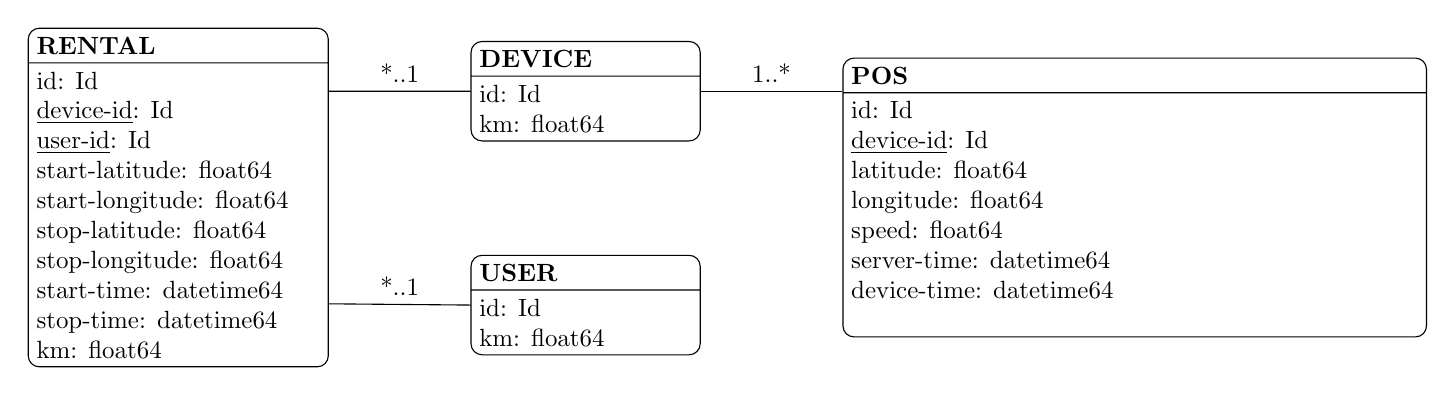
\begin{tikzpicture}[node distance=2cm, scale=0.9, transform shape]
	\node (rental) [rectangle, draw=black, rounded corners, text justified, text width=4cm, rectangle split, rectangle split parts=2]
	{
		\textbf{RENTAL}
		\nodepart{second}
		id: Id\\
		\underline{device-id}: Id\\
		\underline{user-id}: Id\\
		start-latitude: float64\\
		start-longitude: float64\\
		stop-latitude: float64\\
		stop-longitude: float64\\
		start-time: datetime64\\
		stop-time: datetime64\\
		km: float64
	};
	\node (device) [rectangle, draw=black, rounded corners, text justified, text width=3cm, rectangle split, rectangle split parts=2, right=of rental, yshift=1.5cm]
	{
		\textbf{DEVICE}
		\nodepart{second}
		id: Id\\
		km: float64
	};
	\node (pos) [rectangle, draw=black, rounded corners, text justified, text width=8cm, rectangle split, rectangle split parts=2, right=of device, yshift=-1.5cm]
	{
		\textbf{POS}
		\nodepart{second}
		id: Id\\
		\underline{device-id}: Id\\
		latitude: float64\\
		longitude: float64\\
		speed: float64\\
		server-time: datetime64\\
		device-time: datetime64\\
	};
	\node (user) [rectangle, draw=black, rounded corners, text justified, text width=3cm, rectangle split, rectangle split parts=2, below=of device, yshift=0.4cm]
	{
		\textbf{USER}
		\nodepart{second}
		id: Id\\
		km: float64
	};

	\draw ([yshift=1.5cm]rental.east) -- node[above]{*..1}  (device.west);
	\draw ([yshift=-1.5cm]rental.east) -- node[above]{*..1} (user.west);
	\draw (device.east) -- node[above]{1..*} ([yshift=1.5cm]pos.west);
	\end{tikzpicture}
\end{figure*}

\begin{figure*}
	\centering
	\caption{Generated dataset ER model}
	\label{generated-dataset-diagram}
	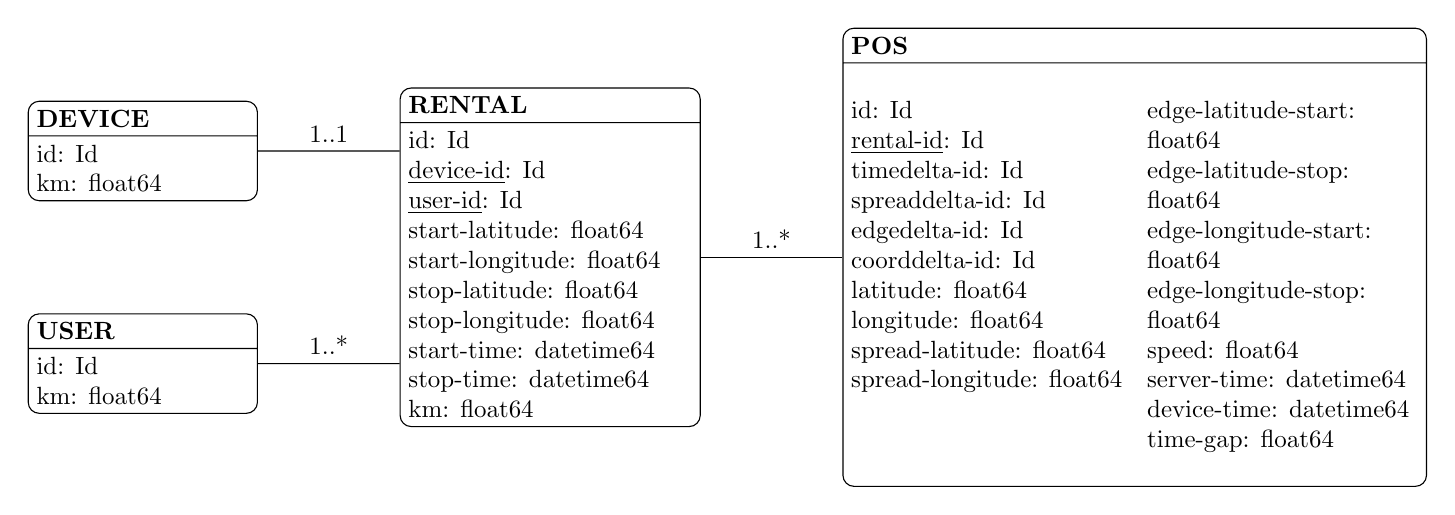
\begin{tikzpicture}[node distance=2cm, scale=0.9, transform shape]
	\node (rental) [rectangle, draw=black, rounded corners, text justified, text width=4cm, rectangle split, rectangle split parts=2]
	{
		\textbf{RENTAL}
		\nodepart{second}
		id: Id\\
		\underline{device-id}: Id\\
		\underline{user-id}: Id\\
		start-latitude: float64\\
		start-longitude: float64\\
		stop-latitude: float64\\
		stop-longitude: float64\\
		start-time: datetime64\\
		stop-time: datetime64\\
		km: float64
	};
	\node (pos) [rectangle, draw=black, rounded corners, text justified, text width=8cm, rectangle split, rectangle split parts=2, right=of rental]
	{
		\textbf{POS}
		\nodepart{second}\begin{multicols*}{2}
		id: Id\\
		\underline{rental-id}: Id\\
		timedelta-id: Id\\
		spreaddelta-id: Id\\
		edgedelta-id: Id\\
		coorddelta-id: Id\\
		latitude: float64\\
		longitude: float64\\
		spread-latitude: float64\\
		spread-longitude: float64\\
		\vfill
		\columnbreak
		edge-latitude-start: float64\\
		edge-latitude-stop: float64\\
		edge-longitude-start: float64\\
		edge-longitude-stop: float64\\
		speed: float64\\
		server-time: datetime64\\
		device-time: datetime64\\
		time-gap: float64\\
		\end{multicols*}
	};
	\node (device) [rectangle, draw=black, rounded corners, text justified, text width=3cm, rectangle split, rectangle split parts=2, left=of rental, yshift=1.5cm]
	{
		\textbf{DEVICE}
		\nodepart{second}
		id: Id\\
		km: float64
	};
	\node (user) [rectangle, draw=black, rounded corners, text justified, text width=3cm, rectangle split, rectangle split parts=2, left=of rental, yshift=-1.5cm]
	{
		\textbf{USER}
		\nodepart{second}
		id: Id\\
		km: float64
	};
	
	\draw ([yshift=1.5cm]rental.west) -- node[above]{1..1}  (device.east);
	\draw ([yshift=-1.5cm]rental.west) -- node[above]{ 1..*} (user.east);
	\draw (rental.east) -- node[above]{1..*} (pos.west);
	\end{tikzpicture}
\end{figure*}

\end{document}
